\documentclass[11pt,a4paper,oneside]{article}
\usepackage[spanish]{babel}
\usepackage[utf8]{inputenc}
\usepackage{olymp}
\usepackage{bnf}
\usepackage{amsfonts}
\usepackage{amsthm}
\newtheorem*{proposition*}{Proposición}
\usepackage{mathtools}
\usepackage{listings}
\usepackage{xcolor}
\definecolor{codegray}{rgb}{0.5,0.5,0.5}
\definecolor{codepurple}{rgb}{0.58,0,0.82}
\definecolor{backcolour}{rgb}{0.95,0.95,0.92}
\lstdefinestyle{mystyle}{
  backgroundcolor=\color{backcolour},
  commentstyle=\color{codepurple}\ttfamily,
  morecomment=[l][\color{magenta}]{\#},
  keywordstyle=\color{blue}\ttfamily,
  numberstyle=\tiny\color{codegray},
  stringstyle=\color{red}\ttfamily,
  basicstyle=\ttfamily,
  breakatwhitespace=false,         
  breaklines=true,                 
  captionpos=b,                    
  keepspaces=true,                 
  numbers=left,                    
  numbersep=5pt,                  
  showspaces=false,                
  showstringspaces=false,
  showtabs=false,                  
  tabsize=2
}
\lstset{style=mystyle}
\usepackage{etoolbox}
\usepackage{graphicx}
\usepackage{wrapfig}
\usepackage{afterpage}
\usepackage{float}
\usepackage[ruled, vlined]{algorithm2e}

\date{Cusco, 29 de Diciembre del 2023}

\renewcommand{\contestname}{
    CusContest XX\\
    Cusco, 29 de Diciembre del 2023
}

\begin{document}

% Provide problems and editorial?
\providetoggle{solution}
% \settoggle{solution}{true}
\settoggle{solution}{false}

\clearpage\thispagestyle{empty}

\begin{figure}
\centering
\begin{minipage}{.32\textwidth}%
    \centering
    
\includegraphics[height=.40\linewidth]{images/logo_hola_google.png}
\end{minipage}%
\begin{minipage}{.32\textwidth}%
    \centering
    
\includegraphics[height=.53\linewidth]{images/logo_acm.png}
\end{minipage}%
\begin{minipage}{.32\textwidth}%
    \centering
    
\includegraphics[height=.22\linewidth]{images/logo_omegaup.png}
\end{minipage}%
\end{figure}

\begin{center}
    \large
    UNIVERSIDAD NACIONAL DE SAN ANTONIO ABAD DEL CUSCO\\
    \vspace{0.3cm}
    FACULTAD DE INGENIERÍA ELÉCTRICA, ELECTRÓNICA, INFORMÁTICA Y MECÁNICA\\
    \vspace{0.3cm}
    ESCUELA PROFESIONAL DE INGENIERÍA INFORMÁTICA Y DE SISTEMAS\\
    \vspace{2cm}
    ACM CHAPTER CUSCO\\
    \vspace{2cm}
    \Large
    CONCURSO DE PROGRAMACIÓN\\
    \vspace{0.5cm}
    \Huge{\textbf{CUSCONTEST XX}\\
    \Large
    \vspace{0.5cm}
    \iftoggle{solution}{\textit{PROBLEMSET CON SOLUCIONES}}{\textit{PROBL3MSET}}
    \\
    \vspace{3cm}
    \large
    Cusco, 29 de Diciembre del 2023\\
    \vspace{3cm}
    Este problemset contiene 13 problemas etiquetados de la `A' a la `M'.
\end{center}

\newpage

\clearpage\thispagestyle{empty}
{\Large \textbf{Información General}}

A menos que se indique lo contrario, las siguientes condiciones son válidas para todos los problemas.


\textbf{Nombre del programa}
\begin{enumerate}
    \item La solución debe ser enviada en formatos del lenguaje seleccionado. Ejm: codigo.c, codigo.cpp, codigo.java, codigo.py, codigo.cs.
\end{enumerate}

\textbf{Entrada}
\begin{enumerate}
    \item La entrada debe ser leída desde la entrada estándar (consola).
    \item La entrada consiste en un único caso de prueba, que es descrito en el formato de cada problema. No existen datos extras en la entrada.
    \item Cuando una línea de datos contiene muchos valores, estos son separados por exactamente un espacio entre ellos. No existen otros espacios en las entradas.
    \item Se utiliza el alfabeto Inglés. No hay letras con tildes, diéresis, eñes, u otros símbolos.
\end{enumerate}

\textbf{Salida}
\begin{enumerate}
    \item La salida debe ser escrita como salida estándar (consola).
    \item El resultado debe ser escrito en la cantidad de líneas especificada para cada problema. No debe imprimirse otros datos. Ejm: no incluir: ``ingrese el número''.
    \item Cuando una línea de datos de salida contiene muchos valores, estos deben ser separados por exactamente un espacio entre ellos. No deben imprimirse otros espacios en las salidas.
    \item Debe ser utilizado el alfabeto Inglés. No letras con tildes, diéresis, eñes, u otros símbolos.
\end{enumerate}

\textbf{Límite de Tiempo}
\begin{enumerate}
    \item El límite de tiempo informado para cada problema corresponde con el tiempo total permitido para la ejecución completa de los casos de prueba.
\end{enumerate}

\textbf{Consejos}
\begin{enumerate}
    \item Para leer múltiples números en una línea en Python usa: A = [int(x) for x in input().split(' ')]
    \item Para soluciones en java, enviar el archivo .java sin el ``package name''.
    \item Para compilar cn c++ y si el archivo se llama code.cpp usar el comando g++ code.cpp -o code y para ejecutar usar el comando ./code
\end{enumerate}

\begin{center}

\vspace{1cm}

Problemas coordinados por Justino Ferro Alvarez, y planteados por:

\vspace{0.3cm}

\begin{tabular}{ l l }
\multicolumn{1}{c}{\textbf{Autor}} & \multicolumn{1}{c}{\textbf{Afiliación}} \\
Ulises Mendez& Software Engineer, Google, USA \\
Erick Alvarez& Software Engineer, Google, USA \\
Rafa Diaz& Canada \& LATAM Community Advisor, Google, CA \\
Grover Castro & PhD in Computer Sc., Universität Leipzig, DE\\
Kleiber Ttito& Software Engineer, Amazon, USA \\
Jared León & PhD Stud. in Maths, University of Warwick, UK\\
John Vargas & Senior Data Scientist, Topaz, USA\\
Josué Nina & Data integration and ETL developer, Provista, USA\\
Justino Ferro & Software Developer, PE\\
\end{tabular}

\end{center}

% Problems come here aquí
\newpage

\begin{problem}{La Rebanada Más Rica}{Entrada estándar}{Salida estándar}{1 segundo}{}{Rafa Diaz}

Todos sabemos bien que por alguna extraña razón la última rebanada de un pan de chuta es la más sabrosa. Por lo mismo las peleas por la última rebanada son bastante férreas.
\\ \\
Tu mejor amiga y tú, para evitar perder la amistad por un pan de chuta, decidieron inventar un juego para decidir quién tomaría esa deliciosa última rebanada.
\\ \\
El juego consiste en imaginariamente dividir el pan en $N$ secciones iguales y usar cada quién un plato que puede contener hasta una rebanada de $M$ secciones de tamaño. A través de un volado deciden quién elige primero una rebanada y toman turnos hasta que alguien se coma la anhelada última rebanada. Las rebanadas que tomen deben medir una cantidad exacta de secciones.
\\\\
Has decidido usar tu arduo entrenamiento en resolución de problemas para desarrollar una estrategia ganadora. Esto no es hacer trampa, por supuesto; sino poner a trabajar esas cientos de horas estudiando en algo de primera importancia: conseguir la anhelada última rebanada.
\\\\
Ahora bien, escribe un programa que dada la cantidad de secciones imaginarias en las que se haya dividido un pan de chuta, la capacidad del plato y quién empieza, diga si es posible garantizar tomar la última rebanada.


\InputFile

En líneas separadas:
\begin{itemize}
    \item Un entero, $N$, indicando la cantidad de secciones imaginarias en las que se divide el pan.
    \item Un entero, $M$, indicando la capacidad máxima del plato, medida en secciones.
    \item $1$ si eres quien empieza, $2$ si no.
\end{itemize}

\textbf{Notas}
\begin{itemize}
    \item $1 \le M \le 1000000$
    \item $1 \le N \le 1000$
\end{itemize}

\OutputFile
\begin{itemize}
    \item `QUE BACAN` si es posible garantizar tomar la última rebanada.
    \item `NO PUEDE SER` si no es posible garantizar tomar la última rebanada.
\end{itemize}


\Example

\begin{example}
\exmp{%%INPUT
2
2
2

}{ %%OUTPUT
NO PUEDE SER
} %%END-OUTPUT


\exmp{%%INPUT
3
1
1

}{ %%OUTPUT
QUE BACAN
} %%END-OUTPUT
\end{example}



Ejemplo 1: Lamentablemente empieza tu amiga y puede tomar una rebanada midiendo $2$ secciones, la última rebanada.

Ejemplo 2: Sólo se pueden tomar rebanadas midiendo $1$ sección. Inevitablemente tomarás la primera y tercera rebanada. Garantizando ganar.

\end{problem}


%%% Local Variables:
%%% mode: latex
%%% TeX-master: "../main"
%%% End:

\iftoggle{solution}{\vspace*{0cm}
{\Large\textbf{Solución}}

\textbf{Conocimientos requeridos:} Matemática básica.

Dados~$a_1, \dots, a_{n-1}$, si el número del niño que desaparece es~$x$, se sabe
que~$a_1 + \cdots + a_{n - 1} + x = 1 + 2 + \cdots + n = n(n + 1) / 2$, por lo
que~$x = n(n + 1) / 2 - (a_1 + \cdots + a_{n - 1})$.

Esta expresión puede ser calculada en~$O(n)$, teniendo la solución una complejidad
final de~$O(tn)$.

\textbf{Implementación en C++:}

\begin{lstlisting}[language=C++]
#include <bits/stdc++.h>
using namespace std;

int main(){
  int te;
  cin >> te;
  while (te--) {
    int n;
    cin >> n;
    int sum = n * (n + 1) / 2;
    for (int i = 0; i < n - 1; i++) {
      int x; cin >> x;
      sum -= x;
    }
    cout << sum << "\n";
  }
  return 0;
}
\end{lstlisting}

\newpage

%%% Local Variables:
%%% mode: latex
%%% TeX-master: "../main"
%%% End:
}{}%
\begin{problem}{Súper Equipo}{Entrada estándar}{Salida estándar}{1 segundo}{}{Rafa Diaz}

Estás de muy buen ánimo al ver que el ACM Chapter Cusco de la Universidad Nacional San Antonio Abad del Cusco crece y crece y que cada vez más y más estudiantes se interesan por temas avanzados de computación.
\\\\
En particular te da alegría ver que cada tema avanzado tiene más de 1 estudiante con amplia experiencia, lo que hará más fácil hacer equipos para el siguiente concurso universitario internacional, el ICPC. Esta observación te ha metido en la cabeza una pregunta que no te deja dormir: ¿cuántas formas posibles hay de elegir los $N$ súper equipos que asistirán al concurso regional?
\\\\
Un súper equipo es un equipo de 3 estudiantes en el que cada quién es experto en uno de los 3 temas que el club considera clave: \emph{programación dinámica}, \emph{grafos} y \emph{matemáticas}.
\\\\
¡Esta noche has decidido desvelarte para crear un programa que calcule la respuesta!
\\\\
Dado el número de estudiantes con amplia experiencia en cada tema encuentra la cantidad de formas en las que se pueden elegir los $N$ súper equipos.

\textbf{Notas:}
\begin{itemize}
    \item Nadie es experto en más de un tema.
    \item No hay jerarquía entre los equipos seleccionados.
\end{itemize}



\InputFile

En líneas separadas:
\begin{itemize}
    \item Un entero, $N$, indicando la cantidad de equipos que se buscan formar.
    \item Un entero, $X$, indicando la cantidad de estudiantes que tienen amplia experiencia en \emph{programación dinámica}
    \item Un entero, $Y$, indicando la cantidad de estudiantes que tienen amplia experiencia en \emph{grafos}
    \item Un entero, $Z$, indicando la cantidad de estudiantes que tienen amplia experiencia en \emph{matemáticas}.
\end{itemize}

\textbf{Notas:}
\begin{itemize}
    \item $1 \le N \le X, Y, Z \le 10$
\end{itemize}

\OutputFile

La cantidad de formas distintas en las que se pueden elegir $N$ súper equipos
\Example

\begin{example}
\exmp{%%INPUT
1
1
2
2

}{ %%OUTPUT
4
} %%END-OUTPUT
\exmp{%%INPUT
2
2
2
3


}{ %%OUTPUT
12
} %%END-OUTPUT
\end{example}



Ejemplo 1:
Llamemos a quien sabe \emph{programación dinámica} $x_1$, a quienes sabe \emph{grafos} $y_1$ y $y_2$, y a quienes saben \emph{matemáticas}: $z_1$ y $z_2$. Si sólo se manda un súper equipo las posibles opciones son: \begin{itemize}
    \item \{$x_1, y_1, z_1$\}
    \item \{$x_1, y_1, z_2$\}
    \item \{$x_1, y_2, z_2$\}
\end{itemize}  
\\

Ejemplpo 2:
Usando la misma nomenclatura del caso anterior, las 12 formas distintas de mandar 2 equipos son:
\begin{itemize}
\item  \{$x_1, y_1, z_1$\} y \{$x_2, y_2, z_2$\}
\item  \{$x_1, y_1, z_2$\} y \{$x_2, y_2, z_3$\}
\item  \{$x_1, y_1, z_3$\} y \{$x_2, y_2, z_1$\}
\item  \{$x_1, y_2, z_1$\} y \{$x_2, y_1, z_2$\}
\item  \{$x_1, y_2, z_2$\} y \{$x_2, y_1, z_3$\}
\item  \{$x_1, y_2, z_3$\} y \{$x_2, y_1, z_1$\}
\item  \{$x_1, y_1, z_1$\} y \{$x_2, y_2, z_3$\}
\item  \{$x_1, y_1, z_2$\} y \{$x_2, y_2, z_1$\}
\item  \{$x_1, y_1, z_3$\} y \{$x_2, y_2, z_2$\}
\item  \{$x_1, y_2, z_1$\} y \{$x_2, y_1, z_3$\}
\item  \{$x_1, y_2, z_2$\} y \{$x_2, y_1, z_1$\}
\item  \{$x_1, y_2, z_3$\} y \{$x_2, y_1, z_2$\}
\end{itemize}
\end{problem}
%%% Local Variables:
%%% mode: latex
%%% TeX-master: "../main"
%%% End:

\iftoggle{solution}{\vspace*{0cm}
{\Large\textbf{Solución}}

\textbf{Conocimientos requeridos:} Arreglos multi-dimensionales (matrices).

El problema requiere una simulación de las reglas~$m$ veces. La implementación es
sencilla pero relativamente larga.

Complejidad~$O(tmn^2)$.

\textbf{Implementación en Python:}

\begin{lstlisting}[language=Python]
import copy
def actualizar(tabla):
    for i in range(N):
        for j in range(N):
            if l[i][j] == 0:
                if (l[i-1][j] + l[i][j-1] + l[(i+1)%N][j] + l[i][(j+1)%N]) in vivoMuert:
                    tabla[i][j] = 1
                else:
                    tabla[i][j] = 0
            else:
                if (l[i-1][j] + l[i][j-1] + l[(i+1)%N][j] + l[i][(j+1)%N]) in vivoReg:
                    tabla[i][j] = 1
                else:
                    tabla[i][j] = 0
    return tabla

for _ in range(int(input())):
    regla_muerto = input()
    regla_vivo = input()
    vivoReg = [-1]*5
    vivoMuert = [-1]*5
    for i in range(5):
        vivoReg[i] = i if regla_vivo[i] == '*' else -1
        vivoMuert[i] = i if regla_muerto[i] == '*' else -1
    N,M = list(map(int,input().split()))
    l = [[0] for i in range(N)]
    for i in range(N):
        l[i] = list(map(int,list([('1' if x == '*' else '0') for x in input()])))
    for _ in range(M):
        l = actualizar(copy.deepcopy(l))
    for i in range(N):
        print (''.join(map(str, [('*' if x == 1 else '.') for x in l[i]])))
\end{lstlisting}

\newpage

%%% Local Variables:
%%% mode: latex
%%% TeX-master: "../main"
%%% End:
}{}%
\begin{problem}{Encuentro Estudiantil Optimizado}{Entrada estándar}{Salida estándar}{1 segundo}{}{Rafa Diaz}

El ACM Chapter Cusco está planeando un Encuentro Estudiantil Nacional el siguiente año. Bien se sabe que un factor importante para llevar a cabo este gran evento es que haya suficientes recursos. Bien se sabe, también, que eres quien sabe más algoritmos de optimización. ¡El Encuentro Estudiantil Nacional te necesita!
\\\\
La tarea que te han asignado es que encuentres la ciudad sede que minimice el costo de transporte de estudiantes que han confirmado su asistencia.
\\\\
Afortunadamente te han dado la siguiente información:
\begin{itemize}
    \item Cantidad de estudiantes que han confirmado su asistencia de cada ciudad.
    \item El costo individual de un boleto de autobús para ir de una ciudad a otra.
\end{itemize}


\InputFile
\begin{itemize}
    \item Un entero, $N$, indicando el número de ciudades.

\item $N$ renglones. Cada renglón seguirá el formato $C E$ donde:
\begin{itemize}
  \item  $C$ representa el nombre de la ciudad (una sola palabra)
  \item  $E$ representa la cantidad de estudiantes confirmados en esa ciudad
  \end{itemize}
\item Un entero, $M$, indicando el número de boletos del que tienes información
\item $M$ renglones. Cada renglón seguirá el formato $C_1 C_2 X$ donde:
\begin{itemize}
    

  \item  $C_1$ y $C_2$ representan las ciudades origen y destino
  \item  $X$ representa el costo en Soles de un boleto individual, ya sea de ida o de regreso
\end{itemize}
\end{itemize}
\textbf{Notas}
\begin{itemize}
\item  $1 \le N \le 20$
\item  $1 \le E_i, X_i \le 100$
\item  Se garantiza que se puede ir de cualquier ciudad a cualquier ciudad
\item  Se garantiza que no hay un par de ciudades con dos costos de un boleto individual
\end{itemize}
\OutputFile

La ciudad que minimiza el costo de transporte de los estudiantes confirmados. En dado caso de empate elige por orden alfabético (e.g. \emph{Cusco} le ganaría a \emph{Puna}).


\Example

\begin{example}
\exmp{%%INPUT
3
Cusco 10
zArequipa 10
Lima 10
3
zArequipa Cusco 20
Cusco Lima 20
zArequipa Lima 20

}{ %%OUTPUT
Cusco
} %%END-OUTPUT

\exmp{%%INPUT
3
Cusco 11
Arequipa 10
Lima 10
3
Arequipa Cusco 20
Cusco Lima 20
Arequipa Lima 20

}{ %%OUTPUT
Cusco
} %%END-OUTPUT
\exmp{%%INPUT
3
Cusco 10
Arequipa 10
Lima 10
3
Arequipa Cusco 20
Cusco Lima 20
Arequipa Lima 21


}{ %%OUTPUT
Cusco
} %%END-OUTPUT
\end{example}




Ejmplo 1: El estimado de transporte de las 3 ciudades es el mismo: 400 Soles. Por lo tanto la ciudad elegida por orden alfabético es \emph{Cusco}.

Ejemplo 2:  Organizar el evento en \emph{Cusco} costaría 400 Soles, mientras que en \emph{Arequipa} o \emph{Lima} sería de 420 Soles


Ejemplo 3: Organizar el evento en \emph{Cusco} costaría 400 Soles, mientras que en \emph{Arequipa} o \emph{Lima} sería de 410 Soles


\end{problem}

%%% Local Variables:
%%% mode: latex
%%% TeX-master: "../main"
%%% End:

\iftoggle{solution}{\vspace*{0cm}
{\Large\textbf{Solución}}

\textbf{Conocimientos requeridos:} Álgebra elemental y descomposición polinómica de un número.

Sea~$n = 1 + \lfloor \log_{10} x \rfloor$ el número de dígitos de~$x$ e~$y$. Sean
también~$x_i$ e~$y_i$ los~$i$-ésimos dígitos más bajos de~$x$ e~$y$ respectivamente,
con indexación~$0$. Luego
\begin{align*}
  xy &= \sum_{i = 0}^{n-1} \sum_{j = 0}^{n-1}x_iy_j 10^{i + j} \\
     &= \sum_{i = 0}^{n-1}x_iy_i 10^{2i} + \sum_{i = 0}^{n-1} \sum_{j = i + 1}^{n -
       1} \left(x_iy_j + x_jy_i\right) 10^{i + j}.
\end{align*}
Es fácil ver que~$\sum_{i = 0}^{n-1}x_iy_i 10^{2i}$ no cambia con las operaciones de
Gándalf. Por lo tanto, el objetivo es
minimizar~$\sum_{i = 0}^{n-1} \sum_{j = i + 1}^{n - 1} \left(x_iy_j + x_jy_i\right)
10^{i + j}$. Para analizar si un intercambio de dígitos vale la pena, se puede
observar que
\begin{equation*}
  \left(x_iy_j + x_jy_i\right) - \left(x_iy_i + x_jy_j\right) = x_i\left(y_j - y_i\right) + x_j\left(y_i - y_j\right) = \left(x_j
    - x_i\right) \left(y_i - y_j\right).
\end{equation*}
Por lo tanto, si~$(x_j - x_i)$ y~$(y_i - y_j)$ tienen el mismo signo (ambos positivos
o ambos negativos), entonces~$x_iy_j + x_jy_i < x_iy_i + x_jy_j$. Si tienen signos
opuestos (uno positivo y el otro negativo),
entonces~$x_iy_i + x_jy_j < x_iy_j + x_jy_i$.

Entonces, para minimizar~$xy$ es conveniente siempre dejar para toda posición~$i$,
que~$x_i$ sea el menor de~$x_i$ e~$y_i$; y que~$y_i$ sea el mayor.

Luego de esto, la respuesta puede ser computada
calculando~$\sum_{i=0}^{n-1}x_i10^{i} \mod 10^9 + 7$
y~$\sum_{i=0}^{n-1}y_i10^{i} \mod 10^9 + 7$ separadamente y luego calculando el
producto de ambos módulo~$10^9 + 7$.

La complejidad por caso de prueba es~$O(n)$, dejando una complejidad total
de~$O(tn)$.

\textbf{Implementación en C++:}

\begin{lstlisting}[language=C++]
#include <bits/stdc++.h>
using namespace std;
const int mod = (int)1e9 + 7;
typedef long long int ll;

int main(){
  int te; cin >> te;
  while (te--) {
    string x, y; cin >> x >> y;
    int n = x.size();
    for (int i = 0; i < n; ++i)
      if(x[i] < y[i]) swap(x[i], y[i]);
    ll xx = 0, yy = 0;
    for (int i = 0; i < n; ++i) {
      xx = (xx * 10 + x[i] - '0') % mod;
      yy = (yy * 10 + y[i] - '0') % mod;
    }
    cout << (xx * yy) % mod << "\n";
  }
  return 0;
}
\end{lstlisting}

\newpage

%%% Local Variables:
%%% mode: latex
%%% TeX-master: "../main"
%%% End:
}{}%
\begin{problem}{Cordilleras}{Entrada estándar}{Salida estándar}{1 segundo}{}{Ulises Mendez Martinez}

\textbf{Antonio} es un entusiasta de las montañas. En su reciente visita a Cuzco y Machu Picchu quedó maravillado por las imponentes vistas que ofrecía la cordillera, así que decidió calcular la altura de las montañas visibles desde cada sitio y guardar dichas mediciones en dos listas (una para cada lugar visitado). En Machu Picchu además, calculó por cada montaña la cantidad de montañas de la primer lista (de Cuzco) cuya altura era estrictamente menor a ella, y formó con esto una tercera lista.

\\ \\

Ya en casa \textbf{Antonio} se dió cuenta de que solo había regresado con la primer y tercer lista, por lo tanto te ha pedido ayuda para reconstruir la segunda lista. \textbf{Antonio} sabe que ninguna montaña medía más de $6385$ metros y que escribió todas las alturas en metros exactos (enteros).


\InputFile

La primer línea de entrada contiene dos enteros separados por un espacio $N, M$ $(1 \le N, M \le 1000)$ que indican la cantidad de montañas en Cuzco y Machu Picchu respectivamente.
La segunda línea contiene $N$ enteros separados por espacios, correspondientes a las alturas $H_i$ $1 \le H_i \le 6385$ de las montañas en el primer sitio.
La tercer y última línea contiene $M$ enteros separados por espacios. En dónde $m_i$ ( $1 \le i \le N$) indica la cantidad de montañas en la primer lista cuya altura es menor a la montaña $i$.

\OutputFile

Una línea con $M$ enteros separados por espacios, que corresponden a la reconstrucción de la segunda lista.

\textbf{Nota1}: En caso de múltiples soluciones, elija aquellas con las mayores alturas.


\textbf{Nota2}: Se garantiza que cada caso tiene al menos una solución.


\Example

\begin{example}
\exmp{%%INPUT
1 1
4444
0
}{ %%OUTPUT
4443
} %%END-OUTPUT
\exmp{%%INPUT
1 1
4444
1
}{ %%OUTPUT
6385
} %%END-OUTPUT
\end{example}



\end{problem}

%%% Local Variables:
%%% mode: latex
%%% TeX-master: "../main"
%%% End:

\iftoggle{solution}{\vspace*{0cm}
{\Large\textbf{Solución}}

\textbf{Conocimientos requeridos:} Ordenamiento.

Se puede almacenar a cada persona en un arreglo o vector, guardando la información
como un par número-cadena (como en un pair\textless int, string\textgreater \, en C++
o una túpla o lista en Python). Al ordenar tal arreglo, la mayoría de los lenguajes
ordena por el primer elemento y luego por el segundo. Por lo tanto, es suficiente
ordenar tal arreglo y mostrar los nombres en tal orden.

La complejidad por caso de prueba es~$O(n\log n)$, dejando una complejidad total
de~$O(tn \log n)$.

\textbf{Implementación en C++:}

\begin{lstlisting}[language=C++]
#include <bits/stdc++.h>
using namespace std;

int main(){
  int te;
  cin >> te;
  while (te--) {
    int n;
    cin >> n;
    vector<pair<int, string>> a(n);
    for(auto &[x, y]: a) cin >> x >> y;
    sort(a.begin(), a.end());
    for(auto [x, gg]: a)
      cout << gg << "\n";
  }
  return 0;
}
\end{lstlisting}

\newpage

%%% Local Variables:
%%% mode: latex
%%% TeX-master: "../main"
%%% End:
}{}%
\begin{problem}{Sendero}{Entrada estándar}{Salida estándar}{1 segundos}{}{Ulises Mendez Martinez}

Se llegó el día de la limpia del sendero que divide el pueblo de \textbf{Antonio} del pueblo vecino. \textbf{Antonio} sabe que dicha actividad genera tensión entre ambas poblaciones, ya que ninguna quiere realizar más trabajo que la otra.

\\ \\

El sendero se representa como una serie de $N$ segmentos continuos partiendo de un pueblo y llegando al otro, cada segmento requiere de un esfuerzo $E_i$ para ser limpiado.

\\ \\

Ayuda a \textbf{Antonio} a calcular cuál es la mayor cantidad de segmentos que se pueden limpiar de manera que cada población realice el mismo esfuerzo acumulado.

\\ \\

\textbf{Nota}: 
Cada población inicia en su lado y no pueden omitir segmentos.


\InputFile

Cada caso de prueba consiste de dos líneas, la primer línea contiene un único entero $N$ $(1 \le N \le 10^3)$, la cantidad de segmentos en el sendero. La segunda línea contiene $N$ enteros separados por un espacio $(E_i, 1\le i \le N)$  con $(1 \le E_i \le 10^6)$, la cantidad de energía requerida por el segmento $i$ para ser limpiado.


\OutputFile

Una línea con dos enteros, indicando la máxima cantidad de segmentos a ser limpiados, la energía acumulada que deberá ser empleada por cada población.

\Example

\begin{example}
\exmp{%%INPUT
3
10 20 10
}{ %%OUTPUT
2 10
} %%END-OUTPUT
\exmp{%%INPUT
6
2 1 4 2 4 1
}{ %%OUTPUT
6 7
} %%END-OUTPUT
\exmp{%%INPUT
5
1 2 4 8 16
}{ %%OUTPUT
0 0
} %%END-OUTPUT
\exmp{%%INPUT
9
7 3 20 5 15 1 11 8 10
}{ %%OUTPUT
7 30
} %%END-OUTPUT
\end{example}





\end{problem}

%%% Local Variables:
%%% mode: latex
%%% TeX-master: "../main"
%%% End:

\iftoggle{solution}{\vspace*{0cm}
{\Large\textbf{Solución}}

\textbf{Conocimientos requeridos:} Teoría de grafos básica y combinatoria.

Dado que Lucho siempre puede comunicarse con todas las otras personas, es fácil ver
que se tiene un grafo conexo. Por lo que cada par de vértices puede conectarse entre
sí. Existen~${n \choose 2} = n(n - 1) / 2$ pares de vértices, siendo ésta la
respuesta siempre.

\textbf{Implementación en C++:}

\begin{lstlisting}[language=C++]
#include <bits/stdc++.h>
using namespace std;

int main(){
  int te;
  cin >> te;
  while (te--) {
    int n, m;
    cin >> n >> m;
    while (m--) {
      int a, b;
      cin >> a >> b;
    }
    cout << (n - 1) * (n - 2) / 2 << "\n";
  }
  return 0;
}
\end{lstlisting}

\newpage

%%% Local Variables:
%%% mode: latex
%%% TeX-master: "../main"
%%% End:
}{}%
\begin{problem}{La Navidad de Kleiber}{Entrada estándar}{Salida estándar}{1 segundo}{}{Kleiber Ttito}

Kleiber es adicto a las compras y especialmente en temporada navideña ya que tiene que dar regalos a todos sus amigos y familiares. Y en la tienda de Amazon durante esta temporada siempre hay una promoción de descuento, donde se puede comprar tres regalos y sólo se paga por dos. Sin embargo, te habrás dado cuenta de que las tiendas que tienen este tipo de promoción son bastante selectivas a la hora de elegir el regalo que obtendras gratis; Siempre son los más baratos.

\\ \\

Por ejemplo, si Kleiber tiene su carrito de compra con siete regalos, que cuestan 400, 350, 300, 250, 200, 150 y 100 soles, tendrá que pagar 1500 soles. En este caso obtuvo un descuento de 250 soles. Pero te das cuenta que si Kleiber separa su compra en tres rondas podría obtener un descuento mayor. Por ejemplo, en la primera ronda se colocaria en el carrito los regalos que cuestan 400, 300 y 250 soles, obteniendo un descuento de 250 soles. En la siguiente ronda el regalo que cuesta 150 soles, no obteniendo ningun descuento adicional. Pero en la tercera ronda se colocaria los últimos regalos que cuestan 350, 200 y 100 soles, obteniendo un descuento de 100 soles adicionales. Sumando todos los descuentos Kleiber podria obrtener un descuento total de 350 soles.

\\\\

Kleiber no puede controlarse a la hora comprar, por lo que pide tú ayuda para encontrar el máximo descuento que puede obtener al comprar los regalos en la tienda de Amazon y asi poder economizar lo máximo posible.

\InputFile

La primera línea de entrada proporciona el número de escenarios, 1 $\leq$ **$t$** $\leq$ 20. Cada escenario consta de dos líneas de entrada. La primera linea indica el número de regalos que Kleiber está comprando, 1 $\leq$ **$n$** $\leq$ 20000. La siguiente línea es la lista de precios de cada uno de los regalos, 1 $\leq$ **$p_i$** $\leq$ 20000.

\OutputFile

Para cada escenario, proporcione en una línea el máximo descuento que Kleiber puede obtener en Amazon eligiendo selectivamente que regalos adiciona al carrito de compras al mismo tiempo.

\Example

\begin{example}
\exmp{%%INPUT
3
7
400 350 300 250 200 150 100
4
10 20 30 40
6
145 172 187 164 135 126
}{ %%OUTPUT
450
20
290
} %%END-OUTPUT
\end{example}

\vspace{0.5cm}


\end{problem}

%%% Local Variables:
%%% mode: latex
%%% TeX-master: "../main"
%%% End:

\iftoggle{solution}{\vspace*{0cm}
{\Large\textbf{Solución}}

\textbf{Conocimientos requeridos:} Arreglos.

Ya que los caracteres serán siempre dígitos, es óptimo siempre el menor de todos los
disponibles hasta agotar las tres pilas.

Complejidad final:~$O(tp_i)$.

\textbf{Implementación en C++:}

\begin{lstlisting}[language=C++]
#include <bits/stdc++.h>
using namespace std;

int main(){
  int te; cin >> te;
  while (te--) {
    int na; cin >> na;
    vector<int> a(na);
    for(auto &e: a) cin >> e;
    int nb; cin >> nb;
    vector<int> b(nb);
    for(auto &e: b) cin >> e;
    int nc; cin >> nc;
    vector<int> c(nc);
    for(auto &e: c) cin >> e;
    na--; nb--; nc--;
    while(na + nb + nc > -3){
      if(na >= 0 && (nb < 0 || (nb >= 0 && a[na] < b[nb])) && (nc < 0 || (nc >= 0 && a[na] < c[nc]))){
        cout << a[na--];
      } else if (nb >= 0 && (na < 0 || (na >= 0 && b[nb] < a[na])) && (nc < 0 || (nc >= 0 && b[nb] < c[nc]))) {
        cout << b[nb--];
      } else{
        cout << c[nc--];
      }
    }
    cout << "\n";
  }
  return 0;
}
\end{lstlisting}

\newpage

%%% Local Variables:
%%% mode: latex
%%% TeX-master: "../main"
%%% End:
}{}%
\begin{problem}{Luces Navideñas de Colores}{Entrada estándar}{Salida estándar}{1 segundo}{}{Grober Castro}

Dado un árbol, donde cada vértice tiene asignado un color (Rojo -'R', Verde - ‘V’). Para cada consulta $(u,v)$, donde $u$ y $v$ son nodos del árbol. Retornar el número de luzes Rojas y Verdes en el camino del nodo $u$ a $v$.


\InputFile

Existen múltiples casos (serán como máximo 10 casos), que finalizan con EOF.
Para cada caso, la primera línea contiene $n$ $(1 \leq n \leq 1000)$  y $q$ $(1 \leq q \leq 20000)$, que representa el número de vértices (enumerados de $1$ a $ n$) y el número de consultas.

Las siguiente línea contiene $n$ caracteres separados por espacios que representan los colores del $i$-ésimo nodo.

Las siguientes $n - 1$ líneas, contiene un par de números enteros $u, v$ $(1 \leq u,v \leq n)$ que representa la existencia de una arista de $u$ a $v$ .

Las siguientes $q$ líneas, contiene dos enteros $u,v $ representando una consulta.

\OutputFile

Para cada consulta debes imprimir el número de nodos de color rojo (R) y verde (V).

\Example

\begin{example}
\exmp{%%INPUT
4 3
R V V R
1 2
2 3
1 4
3 2
2 4
1 3
}{ %%OUTPUT
0 2
2 1
1 2
} %%END-OUTPUT
\end{example}

\end{problem}

%%% Local Variables:
%%% mode: latex
%%% TeX-master: "../main"
%%% End:

\iftoggle{solution}{\vspace*{0cm}
{\Large\textbf{Solución}}

\textbf{Conocimientos requeridos:} Arreglos.

Los límites de este problema impiden verificar todas las pilas cada vez, por lo que
otra estrategia es necesaria. Es posible mantener una cola de prioridad (montículo)
que siempre indique la pila con el menor elemento en el tope. Luego, cada vez que un
elemento es extraído, se puede actualizar el montículo con el tope de la última pila
usada.

Complejidad final:~$O(t\sum_{i=1}^np_i \log \sum_{i=1}^np_i)$.

\textbf{Implementación en C++:}

\begin{lstlisting}[language=C++]
#include <bits/stdc++.h>
using namespace std;

int main() {
  int t;
  cin >> t;
  while (t--) {
    int n; cin >> n;
    stack<int> S[n];
    for (int i = 0; i < n; i++){
      int ss; cin >> ss;
      for (int j = 0; i < ss; j++){
        int a; cin >> a;
        S[i].push(a);
      }
    }
    priority_queue<pair<int,int>> Q;
    for (int i = 0; i < n; i++)
      Q.push({-S[i].top(), i});
    while (!Q.empty()) {
      pair<int, int> curr = Q.top();
      Q.pop();
      cout << -curr.first;
      S[curr.second].pop();
      if(!S[curr.second].empty())
        Q.push({-S[curr.second].top(), curr.second});
    }
    cout << "\n";
  }
  return 0;
}
\end{lstlisting}

\newpage

%%% Local Variables:
%%% mode: latex
%%% TeX-master: "../main"
%%% End:
}{}%
\begin{problem}{Arreglo Rotado}{Entrada estándar}{Salida estándar}{6 segundos}{}{John Vargas}

Encontrar un número en un arreglo ordenado de números únicos que ha sido rotado, un número arbitrario de veces.
Retornar el índice, en el arreglo, del número encontrado.
Retornar $-1$ si el número no existe en el arreglo.

La operación de rotación de un arreglo mueve los números, en el arreglo, como mostrado en el siguiente ejemplo.
Dado el siguiente arreglo: $[2, 4, 5, 6, 9]$
después de rotar a la derecha el arreglo 2 veces obtendremos: $[6, 9, 2, 4, 5]$
  
\InputFile

La primera línea contiene un único número entero $t$ $(1 \leq t \leq 100)$: el número de casos de prueba.

La primera línea de cada caso de prueba contiene un único número entero $n$ $(1 \leq n \leq 10^6)$: el tammaño del arreglo $a$.

Después siguen $n$ lineas que continen los enteros: $a_1,a_2,…,a_n$ $(0 \leq a_i \leq 10^9)$ .

Posteriormente en la siguiente linea sigue un entero $q$ $(1 \leq q \leq 10^7)$ cantidad de consultas.

Por ultimo siguen $q$ lineas de
enteros $v_1,v_2,…,v_q $ $(1 \leq v_i \leq 10^9)$  los números a ser encontrados.

\textbf{Notas}
\begin{itemize}
    \item Asuma que el arreglo no contiene duplicados
\end{itemize}


\OutputFile

Retornar el índice, en el arreglo, del número encontrado caso contrario
retornar $-1$ si el número no existe en el arreglo.

\Example

\begin{example}
\exmp{%%INPUT
2
4
40
100
20
30
2
20
100
2
78
100
1
89
}{ %%OUTPUT
2
1
-1
} %%END-OUTPUT
\end{example}

\textbf{Caso 1:}


Esto por que 20 es el elemento de indice 2 en el arreglo 1 [40, 100, 20, 30]


\textbf{Caso 2:}


100 es el elemento de indice 1 en el arreglo 1 [40, 100, 20, 30]


\textbf{Caso 3:}


$-1$ por que 89 no es un elemento del arreglo 2 [78, 100]


\end{problem}

%%% Local Variables:
%%% mode: latex
%%% TeX-master: "../main"
%%% End:

\iftoggle{solution}{\vspace*{0cm}
{\Large\textbf{Solución}}

\textbf{Conocimientos requeridos:} Arreglos y prefijos.

Es fácil ver que si el rango a tomar es~$[i, j]$, entonces siempre es óptimo
escoger~$p = \min \{t_i, t_{i + 1}, \dots, t_j\}$, y la solución
será~$p (j - i + 1)$. Si para cada posible rango, se calcula el mínimo en tal rango,
entonces es fácil escoger aquel que maximice esta expresión.

El problema ahora se reduce a calcular el mínimo en un rango, para todos los~$O(n^2)$
rangos. Usar una estructura de datos como un Segment Tree (árbol de segmentos) o BIT
(árbol binario indexado) resultará en un Tiempo Límite Excedido. Ya que se quiere
calcular este mínimo para todos los rangos, es posible reutilizar información. Si se
tiene el mínimo para el rango~$[i, j - 1]$, entonces calcular el mínimo para el
rango~$[i, j]$ en tiempo constante es trivial.

La complejidad por caso de prueba es~$O(n^2)$, dejando una complejidad total
de~$O(tn^2)$.

\textbf{Implementación en C++:}

\begin{lstlisting}[language=C++]
#include <bits/stdc++.h>
using namespace std;

int main(){
  int te; cin >> te;
  while (te--) {
    cin >> n;
    vector<int> a(n);
    for(auto &e: a) cin >> e;
    int gg = 0;
    for (int i = 0; i < n; ++i)
      int mini = a[i];
      for (int j = i; j < n; j++) {
        mini = min(mini, a[j]);
        gg = max(gg, mini * (j - i + 1));
      }
    cout << gg << "\n";
  }
  return 0;
}
\end{lstlisting}

\newpage

%%% Local Variables:
%%% mode: latex
%%% TeX-master: "../main"
%%% End:
}{}%
\begin{problem}{Escape de Sobibor}{Entrada estándar}{Salida estándar}{1 segundo}{}{Jared León}

Los Nazis han invadido Polonia y la operación Reinhard está en marcha! Bajo la orden de Himmler, el comandante de la SS, se establecieron cuatro campos de exterminio en el país. Uno de ellos es Sobibor, un campo que retiene pocos cientos de prisioneros vivos de los cientos de miles que pasan por ahí. Sin embargo, hay una pequeña esperanza! Un grupo de prisioneros rebeldes están trabajando en un plan de escape para liberar a todos los prisioneros del lugar.

Los $n$ prisioneros que son parte del plan de escape se encuentran en barracas distintas posicionadas en una línea horizontal en las posiciones $p_1, p_2, \dots, p_n$, (siendo todas distintas). Debido a que un miembro de la SS recorre el complejo cada poco tiempo, el problema actual consiste en encontrar una única localización, dada por una posición $r$ (no necesariamente en una de las barracas) de tal forma que los $n$ prisioneros caminen la mínima distancia total hasta llegar a $r$. Esto da las mejores oportunidades de no ser vistos en el camino. Ayúdales a resolver este problema!

Formalmente, deberás encontrar un entero $r$ tal que la cantidad $|p_1 - r| + |p_2 - r| + ... + |p_n - r|$ sea mínima. Es posible demostrar que existe exactamente un valor que cumple esta condición.
\InputFile

La entrada comienza con un entero $k \leq 10$, indicando el número de casos de prueba. Cada caso de prueba comienza con un entero impar $n$ $(3 \leq n \leq 10^4)$, indicando el número de prisioneros. Cada una de las siguientes $n$ líneas contiene un entero $p_i$ $(0 \leq p_i \leq 10^6)$, indicando la posición del prisionero $i$.

Se garantiza que todos los prisioneros están en posiciones distintas


\OutputFile

Para cada caso de prueba imprime un único entero $r$.
\Example

\begin{example}
\exmp{%%INPUT
3
3
1
5
3
3
6
5
2
5
4
1
8
7
6

}{ %%OUTPUT
3
5
6

} %%END-OUTPUT
\end{example}

\end{problem}

%%% Local Variables:
%%% mode: latex
%%% TeX-master: "../main"
%%% End:

\iftoggle{solution}{\vspace*{0cm}
{\Large\textbf{Solución}}

\textbf{Conocimientos requeridos:} Principio de inclusión-exclusión.

Existen~$\lfloor (n - 1) / x \rfloor$ múltiplos de~$x$
y~$\lfloor (n - 1) / y \rfloor$ múltiplos de~$y$ menores a~$n$. Si se suman estas
cantidades se cuentan los múltiplos de~$x$ e~$y$ dos veces, por lo que es necesario
restar esta cantidad. Ya que~$x$ e~$y$ son números primos, el mínimo común múltiplo
de estos es~$xy$, por lo que existen~$\lfloor (n - 1) / (xy) \rfloor$ múltiplos
de~$xy$ menores que~$n$.

La respuesta
es~$\lfloor (n - 1) / x \rfloor + \lfloor (n - 1) / y \rfloor - \lfloor (n - 1) /
(xy) \rfloor$.

La complejidad por caso de prueba es~$O(1)$, dejando una complejidad total de~$O(t)$.

\textbf{Implementación en C++:}

\begin{lstlisting}[language=C++]
#include <bits/stdc++.h>
using namespace std;
typedef long long int ll;

int main(){
  int te;
  cin >> te;
  while (te--) {
    ll n, x, y;
    cin >> n >> x >> y;
    n--;
    ll gg = n / x + n / y - n / (x * y);
    cout << gg << "\n";
  }
  return 0;
}
\end{lstlisting}

\newpage

%%% Local Variables:
%%% mode: latex
%%% TeX-master: "../main"
%%% End:
}{}%
\begin{problem}{Números Malditos}{Entrada estándar}{Salida estándar}{1 segundo}{}{Justino Ferro}

Luz es una chica muy inteligente y dedicada a sus estudios. Durante su curso de programación competitiva ayer, El profesor planteó un problema intrigante con la siguiente premisa:

Se le pide contar una serie de números, pero con una peculiaridad: debe evitar ciertos números primos que, según la superstición, traen mala suerte. por tal motivo se saltará por completo esos números y sus múltiplos en su conteo. Por ejemplo, si los números primos $3, 5$ y $11$ están en su lista de evitar, la secuencia de números que enumerará comenzará así: $1, 2, 4, 7, 8, 13, 14, 16, 17,. . .$.

El reto consiste en determinar cuál es el $n$-ésimo número en esta secuencia especial. Después de evitar los numero primos y sus múltiplos ¿cuál es el $n$-ésimo número que se obtiene al empezar a contar desde $1$?


El profesor, consciente de la dificultad del problema, mencionó que, además de calificarlo, premiaría con una suma considerable de dinero a la primera persona que lo resolviera.


Motivada por el premio en efectivo y su destreza en matemáticas, Luz encontró rápidamente la idea para la solución del problema y planeó implementarla al llegar a casa.


Cuando estaba a punto de comenzar a implementar la solución, encontró una botella de licor en su casa por casualidad. Aunque supuestamente ella no  bebe alcohol, pensó que era un refresco y se lo tomó. Después de unos minutos, comenzó a sentir los efectos del alcohol y terminó haciendo muchas cosas, excepto resolver el problema.


Hoy es el día de la entrega de la tarea y Luz aún sufre los efectos del alcohol. No ha logrado hacer nada. Dado que este curso es su favorito y no quiere decepcionar a su profesor, te pidió ayuda para implementar la solución al problema.

  
\InputFile

La primera línea de entrada contiene dos números enteros: $n$  $(1 \leq n \leq 10^{17})$, que indica el número de la consulta, y $k$  $(1 \leq k \leq 14)$, que indica el número de números primos distintos que  se evita al contar (de nuevo, también se evitan los múltiplos de estos números primos al contar).

La segunda línea de entrada tiene $k$ números primos distintos, que representan los números (y múltiplos) que se evita.

Supongamos que el producto de todos estos números primos no excederá $10^{17}$, por ejemplo, la lista de números primos puede ser {2, 3, 5, 11} ya que su producto $(330)$ no excede $10^{17}$ pero la lista de números primos no será {1000000007, 1000000009} ya que su producto excede $10^{17}$.



\textbf{Notas:}
\begin{itemize}
    

\item  Tenga en cuenta que, como se muestra en la entrada de ejemplo, los números primos se pueden enumerar en cualquier orden (es decir, no necesariamente se enumeran en orden creciente).
\end{itemize}
\OutputFile

Imprime el $n$-ésimo número que deberá responder Luz  .

\Example

\begin{example}
\exmp{%%INPUT
11 3
3 5 11
}{ %%OUTPUT
23
}
\exmp{%%INPUT
9 4
2 7 3 5
}{ %%OUTPUT
37
}%%END-OUTPUT
\end{example}

\end{problem}

%%% Local Variables:
%%% mode: latex
%%% TeX-master: "../main"
%%% End:

\iftoggle{solution}{\vspace*{0cm}
{\Large\textbf{Solución}}

\textbf{Conocimientos requeridos:} Caminos mínimos en grafos sin peso (BFS) y álgebra
lineal básica.

Por conveniencia, llamaremos a las configuraciones estables simplemente
configuraciones. La siguiente observación es de utilidad para resolver este problema.

\begin{proposition*}
  Dos configuraciones son diferentes si y solo si las suma de los radiovectores de
  los escarabajos en ambas configuraciones son diferentes.
\end{proposition*}
\begin{proof}
Para la condición necesaria, probaremos que una configuración determina únicamente
la suma de los radiovectores de las posiciones. Sea~$(x, y)$ la posición del
escarabajo central en una configuración y las posiciones de los otros
escarabajos~$(x + \Delta x, y)$ y~$(x, y + \Delta y)$. La suma de los radiovectores
de estas posiciones es~$(3x + \Delta x, 3y + \Delta y)$.

Para la condición suficiente, sea~$v$ la suma de los radiovectores de alguna
configuración. No es difícil ver que la posición del escarabajo central es
siempre~$\text{round}(v / 3)$ (donde el redondeo se aplica independientemente a ambas
coordenadas del vector). Teniendo la posición de este escarabajo, es fácil calcular
las posiciones de los demás escarabajos (por ejemplo, si esta posición es~$(x, y)$ y
si la coordenada en~$x$ de~$v$ es~$3x - 1$ entonces hay un escarabajo a la izquierda,
si es~$3x + 1$ hay un escarabajo a la derecha). Por lo tanto, la configuración se
determina únicamente.
\end{proof}

Entonces, el problema se puede replantear como: pasar de la posición~$(1, 1)$ a la
posición~$(x_1 + x_2 + x_3, y_1 + y_2 + y_3)$ saltando de posición en posición de
acuerdo a las reglas de movimiento en el mínimo número de movimientos.

Es posible tratar las posiciones del nuevo problema como vértices de un grafo, donde
el número de vecinos de un vértice es una constante (¿cuál?). El número de vértices y
aristas de este grafo es~$O(\max x_i \max y_i)$ Los límites del problema hacen posible usar el
algoritmo BFS (búsqueda en anchura) en este grafo para encontrar la longitud de un
camino más corto de la posición inicial a la posición final.

La complejidad por caso de prueba es~$O(\max x_i \max y_i)$, dejando una complejidad
total de~$O(t \max x_i \max y_i)$.

Es posible realizar una solución~$O(1)$ por caso de prueba observando un patrón para
posiciones pequeñas y probando que tal patrón se mantiene por inducción.

\textbf{Implementación en C++:}

\begin{lstlisting}[language=C++]
#include <bits/stdc++.h>
using namespace std;

vector<pair<int, int>> adyacentes(int x, int y){
  vector<pair<int, int>> gg;
  int cx = round(x / 3.0), cy = round(y / 3.0);
  int ax = cx + 1, ay = cy;
  if(x == 3 * cx - 1) ax = cx - 1;
  int bx = cx, by = cy + 1;
  if(y == 3 * cy - 1) by = cy - 1;
  // Mover el centro hacia la otra ubic.
  int mx = ax != cx ? ax:bx, my = ay != cy ? ay:by;
  gg.push_back({mx + ax + bx, my + ay + by});
  // Mover a hacia la ubic. 1/3
  mx = ax == cx - 1 ? (cx + 1):(cx - 1);
  my = ay;
  gg.push_back({mx + cx + bx, my + cy + by});
  // Mover a hacia la ubic. 2/3
  my = by;
  gg.push_back({mx + cx + bx, my + cy + by});
  // Mover a hacia la ubic. 3/3
  mx = ax;
  gg.push_back({mx + cx + bx, my + cy + by});
  // Mover b hacia la ubic. 1/3
  mx = bx;
  my = by == cy - 1 ? (cy + 1):(cy - 1);
  gg.push_back({mx + ax + cx, my + ay + cy});
  // Mover b hacia la ubic. 2/3
  mx = ax;
  gg.push_back({mx + ax + cx, my + ay + cy});
  // Mover b hacia la ubic. 3/3
  my = by;
  gg.push_back({mx + ax + cx, my + ay + cy});
  return gg;
}

int main(){
  int te; cin >> te;
  while (te--) {
    int x1, y1, x2, y2, x3, y3;
    cin >> x1 >> y1 >> x2 >> y2 >> x3 >> y3;
    int x = x1 + x2 + x3, y = y = y1 + y2 + y3;

    // BFS
    queue<pair<int, int>> q;
    q.push({1, 1});
    map<pair<int, int>, int> d;
    d[{1, 1}] = 0;
    while (q.size() > 0) {
      pair<int, int> p = q.front(); q.pop();
      int vx = p.first, vy = p.second;
      int dist = d[p];
      for (auto [ux, uy]: adyacentes(vx, vy)) {
        if(d.find({ux, uy}) == d.end() || dist + 1 < d[{ux, uy}]){
          d[{ux, uy}] = dist + 1;
          q.push({ux, uy});
        }
        // Objetivo localizado
        if(ux == x && uy == y){
          queue<pair<int, int>> empty;
          swap(q, empty);
          break;
        }
      }
    }
    cout << d[{x, y}] << "\n";
  }
  return 0;
}
\end{lstlisting}

\newpage

%%% Local Variables:
%%% mode: latex
%%% TeX-master: "../main"
%%% End:
}{}%
\begin{problem}{El Evento Escolar}{Entrada estándar}{Salida estándar}{2 segundo}{}{Erick Alvarez}

Se acerca el evento de fin de año en la Universidad de Cusco y tú eres las persona encargada de llevar a acabo los preparativos previos, para lo que se te ha dado una lista de tareas $T_1$, $T_2$, ..., $T_N$ por cumplir, las cuales a su vez cuentan con una cantidad de subtareas. Ej. la tarea $T_i$ cuenta con las subtareas $t_{i1}$, $t_{i2}$, ..., $t_{ik}$.\\\\

Como eres una persona muy organizada tu has decidido que todas las subtareas asociadas a la tarea $T_i$ se deben cumplir antes de las subtareas asociadas a la tarea $T_{i+1}$ para todo $i$. Para ello decides contar todas las formas en las que esto es posible y anotar el resultado en tu libreta de preparativos.\\\\

\textbf{Aquí va un ejemplo:} Imagina que se tienen las tareas $T_1$, $T_2$ y cada una cuenta con 2 subtareas.
Las maneras en las que podemos organizar estas últimas respetando la restricción anterior es:

$$t_{1}, t_{1}, t_{2}, t_{2}$$

$$t_{1}, t_{2}, t_{1}, t_{2}$$

$$t_{2}, t_{1}, t_{1}, t_{2}$$

Ten en mente que no te importa el orden en el que se realicen las subtareas asociadas a la tarea $T_i$ sólo que estén listas antes de las correspondientes a $T_{i+1}$.

\InputFile

Un número $n$ $(1 \leq n \leq 100)$ indicando la cantidad de tareas a cumplir, en la siguiente línea $n$ enteros  $T_i$ $(0 < T_1 + T_2 + .. + T_n \leq 10^6)$ indicando el número de subtareas asociadas a $T_i$.


\OutputFile

Un único entero indicando el número de formas en las que se pueden cumplir todas las subtareas. Como la salida puede ser muy grande deberás aplicarle módulo \text{1000000007}.


\Example

\begin{example}
\exmp{%%INPUT
2
2 2
}{ %%OUTPUT
3
} %%END-OUTPUT
\exmp{%%INPUT
3
1 2 3
}{ %%OUTPUT
20
} %%END-OUTPUT
\end{example}

\end{problem}

%%% Local Variables:
%%% mode: latex
%%% TeX-master: "../main"
%%% End:

\iftoggle{solution}{\vspace*{0cm}
{\Large\textbf{Solución}}

\textbf{Conocimientos requeridos:} Imprimir en consola.

Este problema no necesita explicación.

\textbf{Implementación en Python:}

\begin{lstlisting}[language=Python]
print(24)
\end{lstlisting}

\newpage

%%% Local Variables:
%%% mode: latex
%%% TeX-master: "../main"
%%% End:
}{}%
\begin{problem}{Puntos Extras}{Entrada estándar}{Salida estándar}{1 segundo}{}{Erick Alvarez}

Este semestre estás tomando el curso de algoritmos y estructuras de datos de la licenciatura y actualmente empezaron a estudiar un tema interesante: compresión de datos. Para ello han visto temas como la \textbf{Codificación Huffman}, sin embargo la última tarea que ha enviado el profesor cuenta con problemas más sencillos, el último de ellos consiste en comprimir una cadena de texto iterándola y por cada conjunto repetido de caracteres deberás contar la cantidad de los mismos y después reemplazar el conjunto por dicha cantidad de caracteres más el caracter original.
\\

Ejemplo: La cadena  \textbf{abbccc} se puede comprimir como \textbf{1a2b3c}.\\

Este reto te resulta muy fácil y lo resuelves en cuestión de minutos. Creyendo que esos eran todos los problemas de la tarea das vuelta a la hoja y miras un enunciado más. Este es una versión más difícil del problema anterior y da 2 puntos adicionales a la tarea si el ejercicio es completado.\\

Ahora, en lugar de considerar la cadena anterior como un todo, esta se deberá dividir en bloques de $k$ elementos contínuos. Por cada bloque se deberán formar los grupos de caracteres, pero además de ello se deberán tomar en cuenta los grupos compuestos de caracteres idénticos en grupos adyacentes a la hora de realizar el conteo final.\\

Si la cadena original es "eoeeuspo" y $k$ es igual a 4 entonces se tienen 2 bloques los cuales se pueden ordenar en "eeeo" y "osup". De esta manera al concatenar las subcadenas y contar el numero de grupos totales el resultado sería 5 (el mínimo posible).\\

¿Crees poder resolver el problema y ganar esos 2 puntos extras?

\InputFile

Una cadena $S$ $(0 < |S| \leq 10^3)$ con letras minúsculas del alfabeto latino y un entero $k$ en la misma línea. Se garantiza que la longitud de la cadena es múltiplo de $k$.

\OutputFile

Un entero, el mínimo número de grupos que se pueden formar.

\Example
\begin{example}
\exmp{%%INPUT
eoeeuspo 4
}{ %%OUTPUT
5
} %%END-OUTPUT

\exmp{%%INPUT
augzqrcddiut 6
}{ %%OUTPUT
10
} %%END-OUTPUT
\end{example}

\end{problem}

%%% Local Variables:
%%% mode: latex
%%% TeX-master: "../main"
%%% End:

\iftoggle{solution}{\vspace*{0cm}
{\Large\textbf{Solución}}

\textbf{Conocimientos requeridos:} Imprimir en consola.

Obviamente la cantidad de dogcoins que necesita Chusky para el país~$i$
es~$d_i / c_i$, lo cual está garantizado de ser entero. La cantidad total necesaria
es la suma de esta expresión para todo~$i$.

La complejidad por caso de prueba es~$O(n)$, dejando una complejidad total
de~$O(t n)$.

\textbf{Implementación en C++:}

\begin{lstlisting}[language=C++]
#include <bits/stdc++.h>
using namespace std;

int main(){
  int te;
  cin >> te;
  while (te--) {
    int n;
    cin >> n;
    int gg = 0;
    while (n--) {
      int ci, di;
      cin >> ci >> di;
      gg += di / ci;
    }
    cout << gg << "\n";
  }
  return 0;
}
\end{lstlisting}

\newpage

%%% Local Variables:
%%% mode: latex
%%% TeX-master: "../main"
%%% End:
}{}%
\begin{problem}{Dios si castiga dos veces}{Entrada estándar}{Salida estándar}{1 segundo}{}{Josue Nina}

Mi amigo Yerim es un gran fanático de la cultura Japonesa, ha invertido años en ello y ya cumple con las característica mas importante para ser considerado un otaku: No bañarse por mas de 3 días.
\end{itemize}
El gran sueño de Yerim es ser parte de un Isekai (un subgénero japonés que involucra personajes transportados a otro mundo, típicamente de fantasía o aventura), el invirtió años construyendo una maquina que permita lograr eso.
Finalmente llego el día en el que pondría a prueba su experimento, pero la maquina falló y como consecuencia lo llevo al pasado, específicamente a la China comunista de 1963.
Ahora Yerim es forzado a trabajar con una remuneración mínima haciendo letreros para el estado, dichos letreros solo pueden ser de dos tipos:
\begin{itemize}
	\item ACM (Asociación de Campesinos Maoístas)
	\item ICPC (Ilustre Colegio de Profesores Comunistas)
\end{itemize}

Yerim recibe una gran cantidad de letras mayúsculas y percibe un beneficio de 5 yuans por cada letrero que forme la palabra: "ACM" o "ICPC".

Cada letra solo puede ser usado en único letrero.


Determinar el máximo beneficio que puede obtener Yerim.

\InputFile
En la primera línea tendrá un entero $t$ $(1 \leq t \leq10^3)$ indicando el número de casos de prueba, las siguientes $t$ líneas tendrá una cadena $s$ ($1\leq |s|\leq200$) que solo contiene letras mayúsculas del alfabeto.


\OutputFile

Para cada caso, imprimir el mayor beneficio que puede obtener Yerim.\\

\Example

\begin{example}
\exmp{%%INPUT
5
IAMCPCC
ACM
ABC
MCAAC
ABCDEFGHIJKLMNOPQRSTUVWKYZ
}{ %%OUTPUT
10
5
0
5
5
} %%END-OUTPUT
\end{example}

\begin{figure}[H]
\centering
  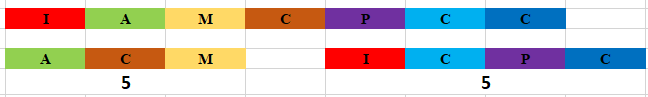
\includegraphics[width=15cm]{images/Screenshot_4.png}
\end{figure}

\end{problem}
\iftoggle{solution}{\vspace*{0cm}
{\Large\textbf{Solución}}

\textbf{Conocimientos requeridos:} Manipulación de cadenas de texto.

Cada palabra debe ser tratada independientemente debido a los espacios. Luego es
suficiente quitar las vocales e imprimir la lista de palabras que no sean vacías
(palabras como ``a'') se convierten en una cadena vacía.

La complejidad por caso de prueba es~$O(|s|)$, dejando una complejidad total
de~$O(t |s|)$.

\textbf{Implementación en Python:}

\begin{lstlisting}[language=Python]
def quitar_vocales(s):
    return ''.join([x for x in s if x not in "aeiou"])

for _ in range(int(input())):
    a = [quitar_vocales(x) for x in input().split(' ')]
    a = [i for i in a if i != ""]
    print(' '.join(a))
\end{lstlisting}

\newpage

%%% Local Variables:
%%% mode: latex
%%% TeX-master: "../main"
%%% End:
}{}%
\begin{problem}{Resta básica }{Entrada estándar}{Salida estándar}{1 segundo}{}{Justino Ferro}

Restando !!!
  
\InputFile

En la primera linea tendrá dos números enteros $a,b$ $(1\leq a,b \leq 10^6)$

\OutputFile
Imprimir el resultado de la resta de los dos números.

\Example

\begin{example}
\exmp{%%INPUT
5 2
}{ %%OUTPUT
3
} %%END-OUTPUT
\exmp{%%INPUT
5 10
}{ %%OUTPUT
-5
} %%END-OUTPUT
\end{example}

Ejemplo1: al primer entero le resto el segundo, y muestro la diferencia

Ejemplo 2: puede haber resultados negativos
\end{problem}

%%% Local Variables:
%%% mode: latex
%%% TeX-master: "../main"
%%% End:

\iftoggle{solution}{\vspace*{0cm}
{\Large\textbf{Solución}}

\textbf{Conocimientos requeridos:} Caminos mínimos en grafos con peso (Dijkstra),
prefijos y sufijos.

Aunque aparentemente la cantidad de cadenas que es necesario verificar es infinita, a
veces es útil pensar en las propiedades matemáticas de algoritmos que nunca terminan.

Supongamos un algoritmo hipotético que intenta construir la cadena final~$s$
concatenando las cadenas dadas desde ambos extremos hacia el centro, probando
potencialmente infinitas configuraciones. Durante su ejecución, supongamos que tal
algoritmo encontró el prefijo~$p = s_{p_1}s_{p_2}\dots s_{p_x}$ y el
sufijo~$q = s_{q_y}s_{q_{y-1}}\dots s_{q_1}$. Si el algoritmo colocó cada cadena sin
permitir que existan colisiones y suponiendo sin pérdida de generalidad
que~$|p| \leq |q|$, entonces los últimos~$|p|$ caracteres de~$q$ forman~$p$ (es
decir,~$p$ es un sufijo de~$q$). Por lo tanto,~$q = r\cdot p$. Más aun, si suponemos
que el algoritmo sólo concatena una nueva cadena con el de menor longitud entre~$p$
y~$q$, entonces~$r$ es el prefijo de alguna cadena dada. Este estado del algoritmo
puede ser representado por el par ordenado~$(\emptyset, r)$ (donde usamos el
símbolo~$\emptyset$ para representar la cadena vacía). Luego, si es posible, el
algoritmo usará una cadena~$s_i$ cuyo prefijo es~$r$ (para no generar una colisión) y
pagará el costo~$c_i$. En el caso en que~$|r| \leq |s_i|$, es decir
que~$s_i = r \cdot t$, entonces el nuevo estado del algoritmo puede ser representado
por~$(t, \emptyset)$. De otra forma, sabemos que~$r = u \cdot s_i$, y el nuevo estado
del algoritmo puede ser representado por~$(\emptyset, u)$.

Con tal representación de los estados de este algoritmo hipotético, es posible
observar que siendo~$s = \max s_i$, solamente existen a lo más~$2ns$ posibles estados
a los que el algoritmo puede llegar (pero infinitos prefijos y sufijos posibles). Por
este motivo, es posible tratar el conjunto

\begin{equation*}
  \{(\emptyset, x): x \text{ es prefijo de algún } s_i\}
  \cup
  \{(x, \emptyset): x \text{ es sufijo no vacío de algún } s_i\}
\end{equation*}

como el conjunto de vértices de un grafo~$G$ cuyas aristas están dadas por la
posibilidad del algoritmo hipotético de moverse de la representación de un estado al
otro y cuyo peso es el costo de usar la cadena que hace posible dicho movimiento. El
número de vértices de~$G$ es~$O(n s)$ y cada vértice tiene grado~$O(n)$, por lo que
el número de aristas es~$O(n^2 s)$. Inicialmente, el algoritmo se encuentra en el
vértice~$(\emptyset, \emptyset)$, y el objetivo es pasar por al menos otro vértice y
llegar a uno de los vértices terminales con el costo mínimo. Claramente, estos
vértices terminales son pares ordenados cuyo término no vacío es un palíndromo y
también el vértice~$(\emptyset, \emptyset)$. Esto puede ser calculado fácilmente con
el algoritmo de Dijkstra.

Con una buena implementación del algoritmo de Dijkstra, la complejidad por caso de
prueba es~$O(|V(G)|\log |V(G)| + |E(G)|) = O(ns(\log(ns) + n))$, dejando una
complejidad total de~$O(tns(n + \log s))$.

\textbf{Implementación en C++:}

\begin{lstlisting}[language=C++]
#include <bits/stdc++.h>
using namespace std;
typedef long long int ll;
const ll oo = 1ll<<60ll;

int main(){
  #ifdef WozMit
  clock_t _start = clock();
  #endif
  int te; cin >> te;
  while (te--) {
    int n; cin >> n;
    vector<string> a(n);
    vector<int> c(n);
    for(auto &e: c) cin >> e;
    for (int i = 0; i < n; ++i)
      cin >> a[i];
    int nn = 0;

    // Identificar todos los vtxs y los terminales
    map<pair<string, string>, int> track;
    vector<int> terminals;
    track[{"", ""}] = nn++;
    for (auto &p: a){
      for (int i = 0; i <= (int)p.size(); ++i){
        if(i > 0){
          string t = p.substr(0, i);
          track[{"", t}] = nn++;
          bool is_pal = true;
          for (int j = 0; is_pal && 2*j < (int)t.size(); j++)
            if(t[j] != t[t.size() - 1 - j]) is_pal = false;
          if(is_pal) terminals.push_back(nn - 1);
        }
        if(i < (int)p.size()){
          string t = p.substr(i);
          track[{t, ""}] = nn++;
          bool is_pal = true;
          for (int j = 0; is_pal && 2*j < (int)t.size(); j++)
            if(t[j] != t[t.size() - 1 - j]) is_pal = false;
          if(is_pal) terminals.push_back(nn - 1);
        }
      }
    }
  
    // Construir el grafo (aristas)
    vector<vector<pair<int, int>>> G(nn);
    for(auto [e, x]: track){
      string t = e.first, s = e.second;
      for (int i = 0; i < n; ++i) {
        bool poss_left = true;
        // Verificar si es posible poner a[i] a la izquierda
        int mini = min(a[i].size(), s.size());
        for (int j = 0; poss_left && j < mini; j++)
          if(a[i][j] != s[s.size() - 1 - j]) poss_left = false;
        if(t != "") poss_left = false;

        bool poss_right = true;
        // Verificar si es posible poner a[i] a la derecha
        mini = min(a[i].size(), t.size());
        for(int j = 0; poss_right && j < mini; j++)
          if(t[j] != a[i][a[i].size() - 1 - j]) poss_right = false;
        if(s != "") poss_right = false;

        if(poss_left){
          if(a[i].size() >= s.size()){
            // Sobra a la izquierda
            pair<string, string> w = {a[i].substr(s.size()), ""};
            int a = x, b = track[w];
            G[a].push_back({b, c[i]});
          } else{
            // Sobra a la derecha
            pair<string, string> w = {"", s.substr(0, s.size() - a[i].size())};
            int a = x, b = track[w];
            G[a].push_back({b, c[i]});
          }
        }
        if(poss_right){
          if(a[i].size() >= t.size()){
            // Sobra a la derecha
            pair<string, string> w = {"", a[i].substr(0, a[i].size() - t.size())};
            int a = x, b = track[w];
            G[a].push_back({b, c[i]});
          } else {
            // Sobra a la izquierda
            pair<string, string> w = {t.substr(a[i].size()), ""};
            int a = x, b = track[w];
            G[a].push_back({b, c[i]});
	  }
	}
      }
    }

    // Ejecutar el algoritmo de Dijkstra's desde 0
    vector<ll> d(nn, oo);
    d[0] = 0;
    priority_queue<pair<ll, int>> q;
    q.push({0, 0});
    while ((int)q.size() > 0) {
      int v = q.top().second;
      ll dv = -q.top().first;
      q.pop();
      // Evitar repetir estados innecesarios
      if(dv != d[v]) continue;
      for(auto edge: G[v]){
        int u = edge.first, w = edge.second;
        if(d[v] + (ll)w < d[u]){
          d[u] = d[v] + (ll)w;
          q.push({-d[u], u});
        }
      }
      // Ya salimos de 0, ya podemos ponerlo en su lugar
      if(v == 0 && d[0] == 0) d[0] = oo;
    }

    ll gg = d[0];
    for (auto e: terminals)
      if(d[e] < gg)
        gg = d[e];
    if(gg == oo) cout << "Imposible\n";
    else cout << gg << "\n";
  }
  return 0;
}
\end{lstlisting}

\newpage

%%% Local Variables:
%%% mode: latex
%%% TeX-master: "../main"
%%% End:
}{}%
\end{document}

%%% Local Variables:
%%% mode: latex
%%% TeX-master: t
%%% End:
